\documentclass[11pt]{article}
\usepackage{enumerate}
\usepackage{fullpage}
\usepackage{fancyhdr}
\usepackage{amsmath, amsfonts, amsthm, amssymb}
\usepackage{color}
\setlength{\parindent}{0pt}
\setlength{\parskip}{5pt plus 1pt}
\usepackage[]{graphicx}
\usepackage{subcaption}

%%%%%%%%%%%%%%%%%%%%%%%HEADER%%%%%%%%%%%%%%%%%%%%%%%%%%%%%%
\newcommand{\myname}{Shashank Singh\footnote{sss1@andrew.cmu.edu}}
\newcommand{\myclass}{36-757 Advanced Data Analysis I}
\newcommand{\myhwname}{ADA Project Summary and Basic EDA}
\newcommand{\duedate}{Friday, January 16, 2015}
%%%%%%%%%%%%%%%%%%%%%%%%%%%%%%%%%%%%%%%%%%%%%%%%%%%%%%%%%%%

%%%%%%%%%%%%%%%%%%%%CONTENT MACROS%%%%%%%%%%%%%%%%%%%%%%%%%
\renewcommand{\qed}{\quad \ensuremath{\blacksquare}}
\newcommand{\inv}{^{-1}}
\newcommand{\bv}{\mathbf{v}}
\newcommand{\bx}{\mathbf{x}}
\newcommand{\by}{\mathbf{y}}
\newcommand{\bff}{\mathbf{f}}
\newcommand{\bzero}{\mathbf{0}}
\newcommand{\bxi}{\boldsymbol{\xi}}
\newcommand{\boldeta}{\boldsymbol{\eta}}
\newcommand{\dist}{\operatorname{dist}}
\newcommand{\area}{\operatorname{area}}
\newcommand{\vspan}{\operatorname{span}}
\newcommand{\Gr}{\operatorname{Gr}} % graph of a function
\renewcommand{\sp}{\operatorname{span}} % span of a set
\newcommand{\sminus}{\backslash}
\newcommand{\E}{\mathbb{E}} % expected value
\newcommand{\F}{\mathcal{F}}
\newcommand{\pr}{\mathbb{P}} % probability
% \newcommand{\Var}{\operatorname{Var}} % variance
\newcommand{\Var}{\mathbb{V}} % variance
\newcommand{\Cov}{\operatorname{Cov}} % covariance
\newcommand{\N}{\mathbb{N}} % natural numbers
\newcommand{\Z}{\mathbb{Z}} % integers
\newcommand{\Q}{\mathbb{Q}} % rational numbers
\newcommand{\R}{\mathbb{R}} % real numbers
\newcommand{\A}{\mathcal{A}}
\newcommand{\B}{\mathcal{B}}
\newcommand{\C}{\mathcal{C}} % compact functions
\newcommand{\K}{\mathbb{K}} % underlying field of a linear space
\newcommand{\Ran}{\mathcal{R}} % range of a linear operator
\newcommand{\Nul}{\mathcal{N}} % null-space of a linear operator
\renewcommand{\L}{\mathcal{L}} % bounded linear functions
\newcommand{\pow}[1]{\mathcal{P}\left(#1\right)} % power set of #1
\newcommand{\e}{\varepsilon} % \varepsilon
\newcommand{\wto}{\rightharpoonup} % weak convergence
\newcommand{\wsto}{\stackrel{*}{\rightharpoonup}} % weak-* convergence
\renewcommand{\P}{\mathbb{P}}   % probability
\newcommand{\ol}{\overline}
%%%%%%%%%%%%%%%%%%%%%%%%%%%%%%%%%%%%%%%%%%%%%%%%%%%%%%%%%%%

\begin{document}
\thispagestyle{plain}

{\Large \myhwname} \\
Name: \myname \\
\myclass \\
Due: \duedate

\section{Project Information}
Internal Advisor: Barnab\'as P\'oczos, Assistant Professor, Machine Learning Department  \\
External Advisor: Timothy Verstynen, Assistant Professor, Psychology Department  \\
Tentatve Title: Inferring Functional Connectivity in Resting State fMRI

Our purpose is to study methods of inferring functional connectivity between
voxels or brain regions during a resting state (i.e., a lack of stimulus).
Questions include whether certain methods, such as Granger causality, that have
been used previously, are in fact primarily measuring artifacts of homeostatic
blood flow (which would be present even during resting state) rather than true
haemodynamic response, as has been suggested by some recent work, and whether
these artefacts can be identified and accounted for when using these methods.
Finally, we would like to compare some more recently proposed methods, such a
information-theoretic aproaches, to see whether they can circumvent this
problem.

\section{Description of Data and Basic EDA}
For each of 24 subjects, the main object of the data is a time series of BOLD
(blood-oxygen-level dependent) signal in each voxel recorded by an fMRI scanner
while subjects were in resting state. Specifically, for each subject, we have a
$V \times T$ matrix, where $V = 160,990$ is the number of voxels and $T = 683$
is the number of time points (sampled at $1$ Hz for 11 minutes and 23 seconds).
The 160,990 voxels comprise $600$ known regions of interest (ROIs), and one way
to reduce the data's dimensionality may be to aggregate data within these ROIs
to produce a $600$ dimensional time series. For each voxel, spatial ($xyz$)
coordinates are also known.

We first perform some basic denoising and normalization on the raw data.
Denoising consists of removing large slow-wave oscillations via PCA by
computing the first $3$ eigenvectors of the signal, reconstructing the signal
from those three eigenvectors, and then substracting the result from the
original signal. We then normalize the data by $Z$-scoring, so that each voxel
has mean $0$ and standard deviation $1$ over time. An example of the resulting
data is given in Figure \ref{fig:eda}.

%%%BEGIN FIGURE%%%
\begin{figure}[h!]
\begin{subfigure}{.5\textwidth}
  \centering
  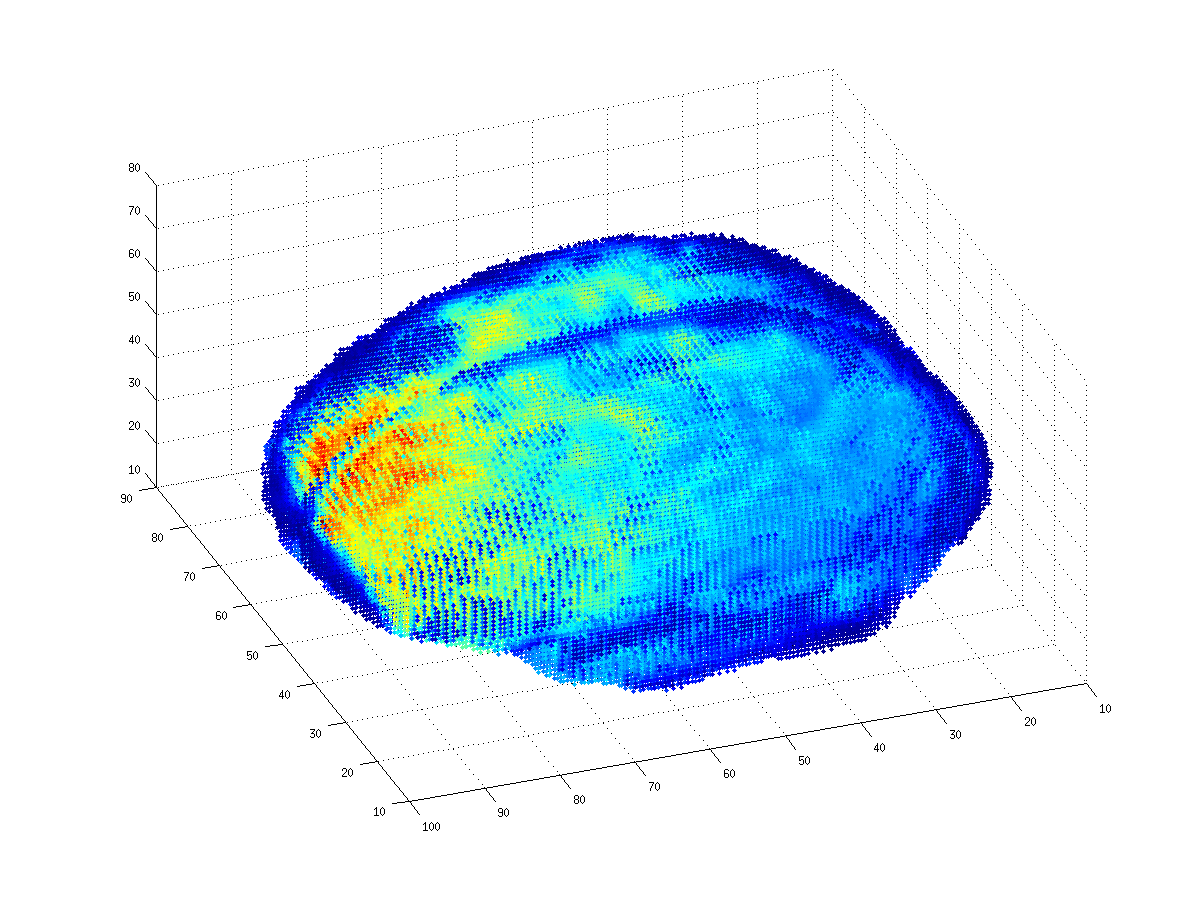
\includegraphics[width=\linewidth]{eda1}
  \caption{1a}
  \label{fig:eda_all}
\end{subfigure}%
\begin{subfigure}{.5\textwidth}
  \centering
  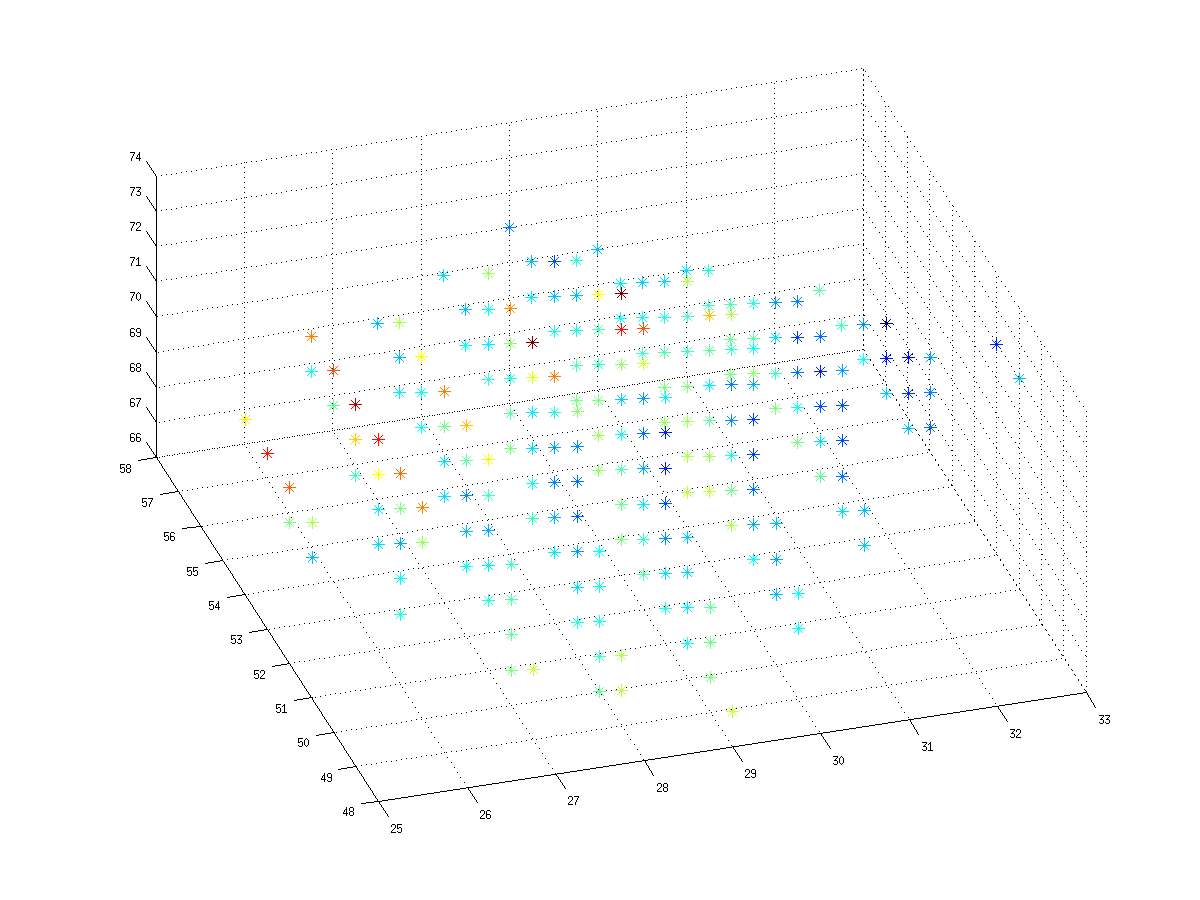
\includegraphics[width=\linewidth]{eda2}
  \caption{1b}
  \label{fig:eda_ROIs}
\end{subfigure}
\caption{BOLD signals for a single time frame from a single subject for all
voxels (\ref{fig:eda_all}) and for all ROIs, averaged over voxels in each ROI
(\ref{fig:eda_ROIs}).}
\label{fig:eda}
\end{figure}
%%%%%END FIGURE%%%

\end{document}
